%++++++++++++++++++++++++++++++++++++++++
% Don't modify this section unless you know what you're doing!
\documentclass[letterpaper,12pt]{article}
\usepackage{tabularx} % extra features for tabular environment
\usepackage{amsmath}  % improve math presentation
\usepackage{graphicx} % takes care of graphic including machinery
\usepackage[margin=1in,letterpaper]{geometry} % decreases margins
\usepackage{cite} % takes care of citations
\usepackage[final]{hyperref} % adds hyper links inside the generated pdf file
\usepackage{pgfplotstable, booktabs}
\usepackage{placeins}
\usepackage{tabularray}
\usepackage{titlesec}
\usepackage{fancyhdr}
\usepackage{empheq}
\usepackage{amssymb}
\usepackage{sectsty}
\usepackage{tcolorbox}
\usepackage{listings}
\usepackage{xcolor}
\usepackage{parskip}
\usepackage{cancel}
\usepackage{enumitem}
\usepackage{amsmath}
\usepackage{mathrsfs}
\usepackage{physics}
\usepackage{subcaption}
\usepackage{float}
% Don't use siunitx for some reason it doesn't work


\definecolor{codegreen}{rgb}{0,0.6,0}
\definecolor{codegray}{rgb}{0.5,0.5,0.5}
\definecolor{codepurple}{rgb}{0.58,0,0.82}

\lstdefinestyle{mystyle}{
    commentstyle=\color{codegreen},
    keywordstyle=\color{codepurple},
    numberstyle=\tiny\color{codegray},
    stringstyle=\color{codegreen},
    basicstyle=\ttfamily\small,
    breakatwhitespace=false,         
    breaklines=true,                 
    captionpos=b,                    
    keepspaces=true,                                                     
    showspaces=false,                
    showstringspaces=false,
    showtabs=false,                  
    tabsize=4
}

\lstset{style=mystyle}
  
\newcommand*\widefbox[1]{\fbox{\hspace{0em}#1\hspace{0em}}}

\pagestyle{fancy}
\fancyhf{} % Clear all header and footer fields
\fancyhead[L]{MEC E 539}
%\fancyhead[C]{Center Header}
\fancyhead[C]{Lab 4}
\fancyhead[R]{Alex Diep}

\fancyfoot[C]{\thepage}

\pgfplotsset{compat=1.18} 
\titleformat*{\section}{\Large\bfseries}
\titleformat*{\subsection}{\large\bfseries}



% \renewcommand{\thesection}{Question \arabic{section}}
% \renewcommand{\thesubsection}{(\alph{subsection})}
\renewcommand*{\arraystretch}{1.5}

\hypersetup{
	colorlinks=true,       % false: boxed links; true: colored links
	linkcolor=blue,        % color of internal links
	citecolor=blue,        % color of links to bibliography
	filecolor=magenta,     % color of file links
	urlcolor=blue         
}

%++++++++++++++++++++++++++++++++++++++++
\begin{document}
\begin{titlepage}
    \centering
    \vspace*{2cm} % Adjust vertical spacing
    
    % Title
    \Huge {MEC E 539 \\Lab 4: Unsteady Laminar Flow Around a Circular Cylinder} \\
    \vspace{1cm} % Adjust vertical spacing
    
    % Author
    \Large by: Alex Diep \\
    \vspace{1cm} % Adjust vertical spacing

    % Date
    \Large Date: March 8, 2024 \\ % or manually specify a date
    \vspace{2cm} % Adjust vertical spacing\
\end{titlepage}

% TOC
\pagenumbering{gobble}
\pagenumbering{roman}
% Table of Contents (Hyperlinks set to locally black)
{
    \hypersetup{hidelinks}
    \tableofcontents
}
\newpage
{
    \hypersetup{linkcolor=black}
    \listoffigures
    \listoftables
}
\newpage
\pagenumbering{arabic}

% Consider laminar flow between two parallel plates (Fig. 1). Plates extend infinitely in x and
% z directions. The following assumptions are made:
% • the flow is at steady state (no time dependency)
% • the fluid is incompressible, ideal and Newtonian
% • the temperature of the bottom plate is Tb and the upper plate is at temperature Tu
% • vy = vz = 0
% • vx = vx(y), T = T(y)
% Figure 1: Problem statement: fluid flow between two parallel plates. The bottom plate is
% fixed, the upper plate is moving horizontally with velocity uw. The fluid is incompressible
% and Newtonian.


\section{}
\textit{Write down the full set of governing equations (continuity, momentum and energy).}

\begin{figure}[h]
    \centering
    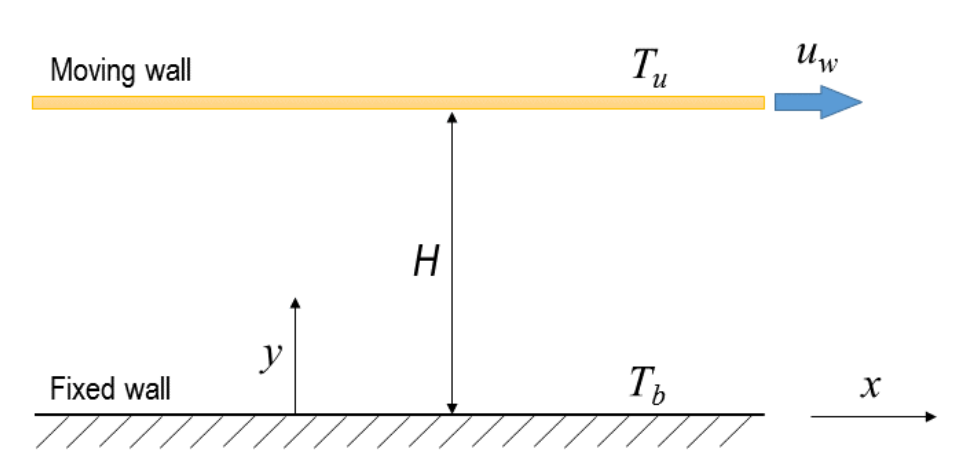
\includegraphics[width=0.5\textwidth]{Questions/Figures/Q1 diagram.png}
    \caption{Fluid flow betweeen parallel plates. The bottom plate is fixed, the upper plate is moving horizontally with velocity $u_w$. THe fluid is incompressible and Newtonian.}
    \label{fig:Q1 diagram}
\end{figure}

\subsection*{Solution}
We first begin with continuity, 
\begin{align*}
    \Aboxed{\frac{\partial \rho}{\partial t} + \vec{u} \cdot \nabla \rho + \rho (\nabla \cdot \vec{u}) &= 0}
\end{align*}
then, the momentum equation,
\begin{align*}
    \Aboxed{\frac{\partial}{\partial t} (\rho u_i) + \frac{\partial}{\partial x_j} (\rho u_i u_j) &= -\frac{\partial P}{\partial x_i} + \frac{\partial}{\partial x_j} \left[ \mu \left( \frac{\partial u_i}{\partial x_j} + \frac{\partial u_j}{\partial x_i} \right) \right] - \frac{\partial}{\partial x_i} \left(\frac{2}{3} \mu \frac{\partial u_k}{\partial x_k} \right) + \rho b_i}
\end{align*}
lastly, the energy equation,
\begin{align*}
    \Aboxed{\rho C_p \left(\frac{\partial T}{\partial t} + \vec{v} \cdot \nabla T \right) &= k \nabla^2 T + \frac{\mu}{2} \Phi^2}
\end{align*}
where $\Phi_{i, j} = \left( \frac{\partial u_i}{\partial x_j} + \frac{\partial u_j}{\partial x_i} \right)$.




\newpage
\bibliographystyle{ieeetr}
\bibliography{references.bib}



\end{document}